\documentclass[semifinal]{cpecmu}

%% This is a sample document demonstrating how to use the CPECMU
%% project template. If you are having trouble, see "cpecmu.pdf" for
%% documentation.

\projectNo{69}%
\acadyear{2020}

\titleTH{เป็นห่วง}%
\titleEN{Penhwang}

\author{นางสาวธนันพร ยานะ}{Tananporn Yana}{600610739}
\author{นายศรัณญ์ ซือสุวรรณ}{Sarun Suesuwan}{600610777}

\cpeadvisor{navadon}
\cpecommittee{chinawat}
\cpecommittee{dome}

%% Some possible packages to include:
\usepackage[final]{graphicx} % for including graphics

%% Add bookmarks and hyperlinks in the document.
\usepackage[colorlinks=true,allcolors=Blue4,citecolor=red,linktoc=all]{hyperref}

%% Needed just by this example, but maybe not by most reports
\usepackage{afterpage} % for outputting
\usepackage{pdflscape} % for landscape figures and tables. 

%% Some other useful packages. Look these up to find out how to use
%% them.
% \usepackage{natbib}    % for author-year citation styles
% \usepackage{txfonts}
% \usepackage{appendix}  % for appendices on a per-chapter basis
% \usepackage{xtab}      % for tables that go over multiple pages
% \usepackage{subfigure} % for subfigures within a figure
% \usepackage{pstricks,pdftricks} % for access to special PostScript and PDF commands
% \usepackage{nomencl}   % if you have a list of abbreviations

%% if you're having problems with overfull boxes, you may need to increase
%% the tolerance to 9999
% \tolerance=9999

\bibliographystyle{plain}
% \bibliographystyle{IEEEbib}

% \renewcommand{\topfraction}{0.85}
% \renewcommand{\textfraction}{0.1}
% \renewcommand{\floatpagefraction}{0.75}

%% Example for glossary entry
%% Need to use glossary option
%% See glossaries package for complete documentation.
\ifglossary
  \newglossaryentry{lorem ipsum}{
    name=lorem ipsum,
    description={derived from Latin dolorem ipsum, translated as ``pain itself''}
  }
\fi

%% Uncomment this command to preview only specified LaTeX file(s)
%% imported with \include command below.
%% Any other file imported via \include but not specified here will not
%% be previewed.
%% Useful if your report is large, as you might not want to build
%% the entire file when editing a certain part of your report.
% \includeonly{chapters/intro,chapters/background}

\begin{document}
\maketitle
\makesignature

\ifproject
\begin{abstractTH}

เนื่องจากในปัจจุบันบริษัทหลาย ๆ แห่งเริ่มใช้แอปพลิเคชันเพื่อทำการบันทึกเวลาเข้า-ออกของพนักงาน แทนการบันทึกโดยใช้กระดาษ, บัตรตอก หรือ เครื่องสแกนนิ้วมือ
\enskip เพื่อความรวดเร็วในการดึงข้อมูลมาแสดง และ ความยืดหยุ่นในการเลือกเวลาทำงานของพนักงาน
\enskip แต่แอปพลิเคชันต่าง ๆ เหล่านี้ก็ยังมีข้อเสียบางประการเช่น ไม่ค่อยมีการแจ้งเตือนพนักงาน ทำให้แอปดูห่างเหินกับพนักงาน, 
การลงชื่อเข้าหรือออกยังทำได้ยาก มีหลายขั้นตอน ทำให้เวลาที่บันทึกเข้าสู่ระบบกับเวลาที่พนักงานเข้างานจริงต่างกันพอสมควร 
และ ในบางครั้งอุปกรณ์ของพนักงานอาจไม่มีพื้นที่เพียงพอที่จะดาวน์โหลดแอปพลิเคชันนั้น ๆ
\enskip เพื่อลดข้อเสียเหล่านี้ทางเราจึงได้พัฒนา เป็นห่วง ซึ่งเป็นไลน์แชทบอทที่ต่อยอดให้สามารถทำงานต่าง ๆ ของแอปพลิเคชันซึ่งกล่าวมาข้างต้นได้
แต่สามารถแก้ข้อเสียที่เกิดขึ้นได้ เช่น สามารถแจ้งเตือนได้ สามารถเข้าถึงได้ง่าย และ ไม่ต้องดาวน์โหลดแอปพลิเคชันเพิ่มเติม
\end{abstractTH}


\begin{abstract}
Nowadays, many companies began to use an application to record time attendance of employees instead of note in paper, punch card or finger scanner 
for speed up access to information and increased flexibility in choosing the working hours of employees.
\end{abstract}

\iffalse
\begin{dedication}
This document is dedicated to all Chiang Mai University students.

Dedication page is optional.
\end{dedication}
\fi % \iffalse

\begin{acknowledgments}
Your acknowledgments go here. Make sure it sits inside the
\texttt{acknowledgment} environment.

\acksign{2020}{5}{25}
\end{acknowledgments}%
\fi % \ifproject

\contentspage

\ifproject
\figurelistpage

\tablelistpage
\fi % \ifproject

% \abbrlist % this page is optional

% \symlist % this page is optional

% \preface % this section is optional


\pagestyle{empty}\cleardoublepage
\normalspacing \setcounter{page}{1} \pagenumbering{arabic} \pagestyle{cpecmu}

\chapter{\ifcpe บทนำ\else Introduction\fi}

\section{\ifcpe ที่มาของโครงงาน\else Project rationale\fi}
บริษัทต่าง ๆ ที่มีพนักงานและมีการจ่ายเงินเดือนตามเวลาเข้าออกงานของพนักงานก็จะมีวิธีการเช็คชื่อเข้า-ออกงานของพนักงานที่ต่างกัน 
หลากหลายรูปแบบ เช่น การเซ็นชื่อลงบนกระดาษ, การตอกบัตร หรือ การสแกนลายนิ้วมือ
แต่ในปัจจุบันมีบริษัทส่วนหนึ่งได้ตระหนักถึงปัญหาจากการใช้วิธีการเช็คชื่อเข้าออกงานแบบเดิม ๆ 
เช่น คำนวณเงินเดือนยากเพราะต้องทำการค้นหาข้อมูลจากเอกสารจำนวนมาก 
พนักงานทุจริตด้วยการตอกบัตรแทนกัน 
หรือ พนักงานตอกบัตรผิดใบ 
ซึ่งการใช้มนุษย์ในการบันทึกหรือจัดการข้อมูล มักจะเกิดความผิดพลาดที่เกิดจากมนุษย์(human error) 
และเกิดความล่าช้า โดยจะสังเกตได้จากในวันออกเงินเดือน พนักงานจะได้กลับบ้านช้ากว่าปกติเพราะต้องรอคำนวณเงินเดือนให้เสร็จเสียก่อน

จึงมีบริษัทส่วนหนึ่งเลือกที่จะใช้แอปพลิเคชันต่าง ๆ เพื่อที่จะจัดการแก้ไขปัญหาดังกล่าวข้างต้น 
เพราะสามารถเรียกดูข้อมูลได้ตลอดเวลา 
สรุปผลและคำนวณออกมาเป็นเงินเดือนได้อย่างรวดเร็ว 
สามารถป้องกันการทุจริตของพนักงาน 
รวมไปถึงจัดการการเดินเรื่องขอเอกสารให้มีความสะดวกรวดเร็วมากยิ่งขึ้น และ ลดปัญหาที่เกิดขึ้นจากการเก็บข้อมูลโดยใช้มนุษย์ไปพร้อมกัน

แต่แอปพลิเคชันเหล่านี้ก็ยังมีข้อเสีย เช่น 
พนักงานต้องทำการดาวน์โหลดแอปพลิเคชันไว้ในเครื่องส่วนตัวซึ่งพนักงานส่วนใหญ่ไม่เต็มใจที่จะดาวน์โหลดแอป โดยบางแอปพลิเคชันไม่ได้อำนวยความสะดวกในการใช้งานด้านต่าง ๆ เช่น
ไม่มีการแจ้งเตือนเมื่อพนักงานจะต้องเข้าทำงาน, กำลังจะเข้างานสาย, มีการเปลี่ยนแปลงเวลาการทำงานของตนเอง หรือ คำขอต่าง ๆ ของตนเองถูกยืนยัน/ปฎิเสธ
ซึ่งเป็นสิ่งที่แอปพลิเคชันควรจะรองรับ 
และการเช็คชื่อเข้าทำงานของพนักงานยังทำได้ช้าและมีหลายขั้นตอนทำให้เวลาที่บันทึกอยู่ในระบบและเวลาที่พนักงานเข้างานจริงต่างกันพอสมควร

ทางผู้พัฒนาเล็งเห็นปัญหาข้างต้นจึงได้พัฒนาโปรเจคนี้ขึ้นโดยการใช้ line chatbot มาพัฒนาต่อยอด
เพื่อให้สามารถทำงานตามที่แอปพลิเคชันเหล่านั้นทำได้
โดยรักษาข้อดีต่าง ๆ เอาไว้ และ แก้ปัญหาที่เกิดขึ้นจากการใช้แอปพลิเคชันเหล่านั้นด้วย

\section{\ifcpe วัตถุประสงค์ของโครงงาน\else Objectives\fi}
\begin{enumerate}
    \item พัฒนาแชทบอทที่สามารถทำงานหลัก ๆ ของแอปพลิเคชันเช็คชื่อพนักงานได้ คือ 
    \begin{enumerate}
    \item[1.1] จัดตารางเข้า-ออกให้กับพนักงานที่อยู่ในสายบังคับของตน
    \item[1.2] เช็คชื่อเข้า-ออกโดยใช้การถ่ายรูป พร้อมกับตรวจสอบที่อยู่ 
    \item[1.3] สามารถยื่นคำขอเปลี่ยนเวลาการทำงานของตนเอง
    \item[1.4] ตั้งค่าบริษัทเช่น การเพิ่ม-ลดพนักงาน และ สายบังคับของพนักงาน 
    \end{enumerate} 
    \item มีการแจ้งเตือนเมื่อพนักงานจะต้องเข้าทำงาน, กำลังจะเข้างานสาย, มีการเปลี่ยนแปลงเวลาการทำงานของตนเอง หรือ คำขอต่าง ๆ ของตนเองถูกยืนยัน/ปฎิเสธ
    \item ต้องเป็น chatbot ที่คุยด้วยแล้วเหมือนคุยกับคนจริง ๆ ที่กำลังหาข้อมูลมาตอบ/ทำเรื่องอยู่
\end{enumerate}

\section{\ifcpe ขอบเขตของโครงงาน\else Project scope\fi}

\subsection{\ifcpe ขอบเขตด้านฮาร์ดแวร์\else Hardware scope\fi}
\begin{itemize}
    \item Android version 4.4 เป็นต้นไป
\end{itemize}

\subsection{\ifcpe ขอบเขตด้านซอฟต์แวร์\else Software scope\fi}
\begin{itemize}
    \item ระบบบันทึกเวลาการเข้าออกงานของพนักงาน
    \item ระบบจัดการตารางเวลาทำงาน 
    \item ระบบแจ้งเตือนก่อนเวลาเข้างาน
    \item ระบบแจ้งเตือนเมื่อมีการเปลี่ยนแปลงตารางเวลาการทำงาน
    \item ระบบแจ้งเตือนเมื่อมีการอนุมัติ/ปฏิเสธคำของต่าง ๆ
    \item ระบบคำนวณเงินเดือน
\end{itemize}

\section{\ifcpe ประโยชน์ที่ได้รับ\else Expected outcomes\fi}
\begin{itemize}
    \item ช่วยอำนวยความสะดวกในการบันทึกเวลาเข้าออกงาน
    \item บันทึกข้อมูลไว้เพื่อง่ายต่อการตรวจสอบ
    \item ใช้เวลาในการจัดการเอกสารคำขอต่าง ๆ น้อยลง
    \item สามารถดูสิทธิ์การลาคงเหลือ และสรุปประวัติการบันทึกเวลาได้ง่ายและทันที
    \item หัวหน้างานสามารถติดตามการเข้าออกงานของลูกน้องได้แบบ Real-Time
    \item มีระบบการแจ้งเตือนทำให้สามารถจัดการหรือเตรียมตัวก่อนล่วงหน้า
\end{itemize}
\section{\ifcpe เทคโนโลยีและเครื่องมือที่ใช้\else Technology and tools\fi}
\begin{itemize}
    \item VS code
    \item Line application
    \item Line API Messenging
    \item Line Bot Designer​ \end{englang}
    \item Dialogflow
    \item firebase
    \item Nuxt.js
\end{itemize}
\section{\ifcpe แผนการดำเนินงาน\else Project plan\fi}
\begin{plan}{7}{2020}{3}{2021}
    \planitem{7}{2020}{9}{2020}{ศึกษาแอปฯปัจจุบัน}
    \planitem{8}{2020}{9}{2020}{ศึกษาการสร้างแชทบอท​}
    \planitem{7}{2020}{9}{2020}{ออกแบบระบบ}
    \planitem{10}{2020}{10}{2020}{ออกแบบแชทบอท​}
    \planitem{7}{2020}{10}{2020}{ออกแบบเว็บ​}
    \planitem{7}{2020}{10}{2020}{ออกแบบฐานข้อมูล}
    \planitem{11}{2020}{12}{2020}{สร้างแชทบอท}
    \planitem{11}{2020}{1}{2021}{เชื่อมแชทบอทกับฐานข้อมูล}
    \planitem{11}{2020}{1}{2021}{สร้างเว็บ}
    \planitem{11}{2020}{2}{2021}{เชื่อมเว็บกับแชทบอท}
    \planitem{11}{2020}{3}{2021}{ทดสอบและแก้ไข Bugs}
\end{plan}

\section{\ifcpe บทบาทและความรับผิดชอบ\else Roles and responsibilities\fi}
\begin{itemize}
    \item น.ส.ธนันพร ยานะ
    \begin{itemize}
        \item Web designer​ \end{englang}
        \item Chatbot designer​​ \end{englang}
        \item Frontend developer​ \end{englang}
    \end{itemize}
    \item นายศรัณญ์ ซือสุวรรณ
    \begin{itemize} 
        \item Database admin
        \item Backend developer​​ \end{englang}
    \end{itemize}
\end{itemize}

\section{\ifcpe%
ผลกระทบด้านสังคม สุขภาพ ความปลอดภัย กฎหมาย และวัฒนธรรม
\else%
Impacts of this project on society, health, safety, legal, and cultural issues
\fi}

แนวทางและประโยชน์ในการประยุกต์ใช้งานโครงงานกับงานในด้านอื่นๆ รวมถึงผลกระทบในด้านสังคมและสิ่งแวดล้อมจากการใช้ความรู้ทางวิศวกรรมที่ได้

\chapter{\ifcpe ทฤษฎีที่เกี่ยวข้อง\else Background Knowledge and Theory\fi}

การทำโครงงาน เริ่มต้นด้วยการศึกษาค้นคว้า ทฤษฎีที่เกี่ยวข้อง หรือ งานวิจัย/โครงงาน ที่เคยมีผู้นำเสนอไว้แล้ว ซึ่งเนื้อหาในบทนี้ก็จะเกี่ยวกับการอธิบายถึงสิ่งที่เกี่ยวข้องกับโครงงาน เพื่อให้ผู้อ่านเข้าใจเนื้อหาในบทถัดๆ ไปได้ง่ายขึ้น

\section{The first section}
The text for Section 1 goes here.

\section{Second section}
Section 2 text.

\subsection{Subsection heading goes here}

Subsection 1 text

\subsubsection{Subsubsection 1 heading goes here}
Subsubsection 1 text

\subsubsection{Subsubsection 2 heading goes here}
Subsubsection 2 text

\section{Third section}
Section 3 text. The dielectric constant\index{dielectric constant}
at the air-metal interface determines
the resonance shift\index{resonance shift} as absorption or capture occurs
is shown in Equation~\eqref{eq:dielectric}:

\begin{equation}\label{eq:dielectric}
k_1=\frac{\omega}{c({1/\varepsilon_m + 1/\varepsilon_i})^{1/2}}=k_2=\frac{\omega
\sin(\theta)\varepsilon_\mathit{air}^{1/2}}{c}
\end{equation}

\noindent
where $\omega$ is the frequency of the plasmon, $c$ is the speed of
light, $\varepsilon_m$ is the dielectric constant of the metal,
$\varepsilon_i$ is the dielectric constant of neighboring insulator,
and $\varepsilon_\mathit{air}$ is the dielectric constant of air.

\section{About using figures in your report}

% define a command that produces some filler text, the lorem ipsum.
\newcommand{\loremipsum}{
  \textit{Lorem ipsum dolor sit amet, consectetur adipisicing elit, sed do
  eiusmod tempor incididunt ut labore et dolore magna aliqua. Ut enim ad
  minim veniam, quis nostrud exercitation ullamco laboris nisi ut
  aliquip ex ea commodo consequat. Duis aute irure dolor in
  reprehenderit in voluptate velit esse cillum dolore eu fugiat nulla
  pariatur. Excepteur sint occaecat cupidatat non proident, sunt in
  culpa qui officia deserunt mollit anim id est laborum.}\par}

\begin{figure}
  \centering

  \fbox{
     \parbox{.6\textwidth}{\loremipsum}
  }

  % To include an image in the figure, say myimage.pdf, you could use
  % the following code. Look up the documentation for the package
  % graphicx for more information.
  % \includegraphics[width=\textwidth]{myimage}

  \caption[Sample figure]{This figure is a sample containing \gls{lorem ipsum},
  showing you how you can include figures and glossary in your report.
  You can specify a shorter caption that will appear in the List of Figures.}
  \label{fig:sample-figure}
\end{figure}

Using \verb.\label. and \verb.\ref. commands allows us to refer to
figures easily. If we can refer to Figures
\ref{fig:walrus} and \ref{fig:sample-figure} by name in the {\LaTeX}
source code, then we will not need to update the code that refers to it
even if the placement or ordering of the figures changes.

\loremipsum\loremipsum

% This code demonstrates how to get a landscape table or figure. It
% uses the package lscape to turn everything but the page number into
% landscape orientation. Everything should be included within an
% \afterpage{ .... } to avoid causing a page break too early.
\afterpage{
  \begin{landscape}
  \begin{table}
    \caption{Sample landscape table}
    \label{tab:sample-table}

    \centering

    \begin{tabular}{c||c|c}
        Year & A & B \\
        \hline\hline
        1989 & 12 & 23 \\
        1990 & 4 & 9 \\
        1991 & 3 & 6 \\
    \end{tabular}
  \end{table}
  \end{landscape}
}

\loremipsum\loremipsum\loremipsum

\section{Overfull hbox}

When the \verb.semifinal. option is passed to the \verb.cpecmu. document class,
any line that is longer than the line width, i.e., an overfull hbox, will be
highlighted with a black solid rule:
\begin{center}
\begin{minipage}{2em}
juxtaposition
\end{minipage}
\end{center}

\section{\ifcpe%
ความรู้ตามหลักสูตรซึ่งถูกนำมาใช้หรือบูรณาการในโครงงาน
\else%
ISNE knowledge used, applied, or integrated in this project
\fi
}

อธิบายถึงความรู้ และแนวทางการนำความรู้ต่างๆ ที่ได้เรียนตามหลักสูตร ซึ่งถูกนำมาใช้ในโครงงาน

\section{\ifcpe%
ความรู้นอกหลักสูตรซึ่งถูกนำมาใช้หรือบูรณาการในโครงงาน
\else%
Extracurricular knowledge used, applied, or integrated in this project
\fi
}

อธิบายถึงความรู้ต่างๆ ที่เรียนรู้ด้วยตนเอง และแนวทางการนำความรู้เหล่านั้นมาใช้ในโครงงาน

\chapter{\ifproject%
\ifcpe โครงสร้างและขั้นตอนการทำงาน\else Project Structure and Methodology\fi
\else%
\ifcpe โครงสร้างของโครงงาน\else Project Structure\fi
\fi
}

ในบทนี้จะกล่าวถึงหลักการ และการออกแบบระบบ

\makeatletter

% \renewcommand\section{\@startsection {section}{1}{\z@}%
%                                    {13.5ex \@plus -1ex \@minus -.2ex}%
%                                    {2.3ex \@plus.2ex}%
%                                    {\normalfont\large\bfseries}}

\makeatother
%\vspace{2ex}
% \titleformat{\section}{\normalfont\bfseries}{\thesection}{1em}{}
% \titlespacing*{\section}{0pt}{10ex}{0pt}

\section{แผนการทำงาน}
\quad ใช้รูปแบบ Software Development Models เป็นรูปแบบ Scrum โดยแบ่งการทำงานเป็น Sprint  โดยที่แต่ละ Sprint มีระยะเวลา 1 สัปดาห์ ในแต่ละสัปดาห์ในช่วงท้ายของสัปดาห์จะมีการตรวจสอบความคืบหน้าของการดำเนินงานในส่วนต่าง ๆ และทุก ๆ ท้ายของ Sprint จะมีการประชุมทบทวนแผนงานที่จะทำสำหรับ Sprint ถัดไปร่วมกันเพื่อยืนยันแผนการดำเนินงานหากมีการเปลี่ยนแปลงเกิดขึ้น 
\section{การทำงานของระบบ}
\begin{figure}
\begin{center}
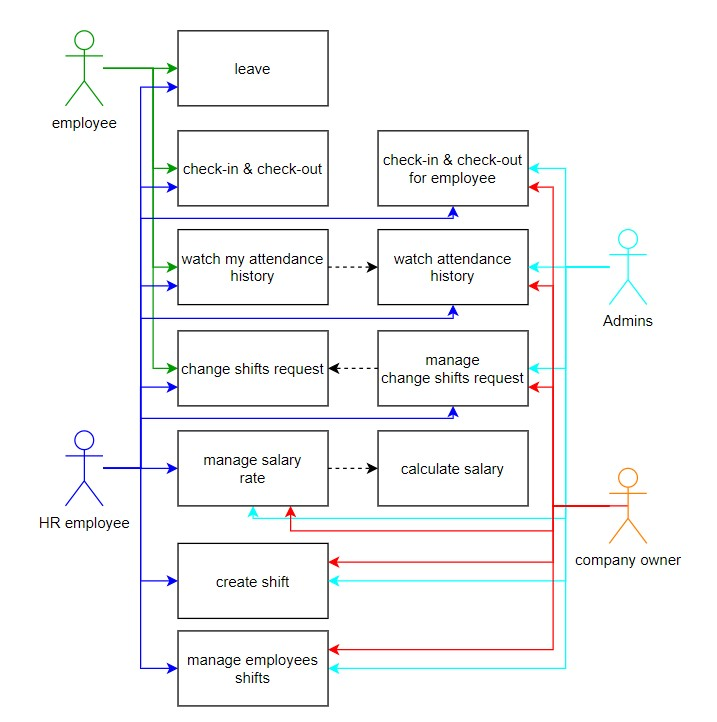
\includegraphics[width=14cm,keepaspectratio]{./images/usecaseDiagram.jpg}
\end{center}
\caption[Poem]{แสดง use case diagram ซึ่งแสดงให้เห็นกลุ่มผู้ใช้งานทั้ง 4 กลุ่มประกอบด้วย พนักงานทั่วไป(employee), พนักงานHR(HRemployee), เจ้าของกิจการ(company owner) และ admin รวมถึง function ที่ผู้ใช้กลุ่มนั้นใช้งานได้}
\end{figure}

\begin{figure}
\begin{center}
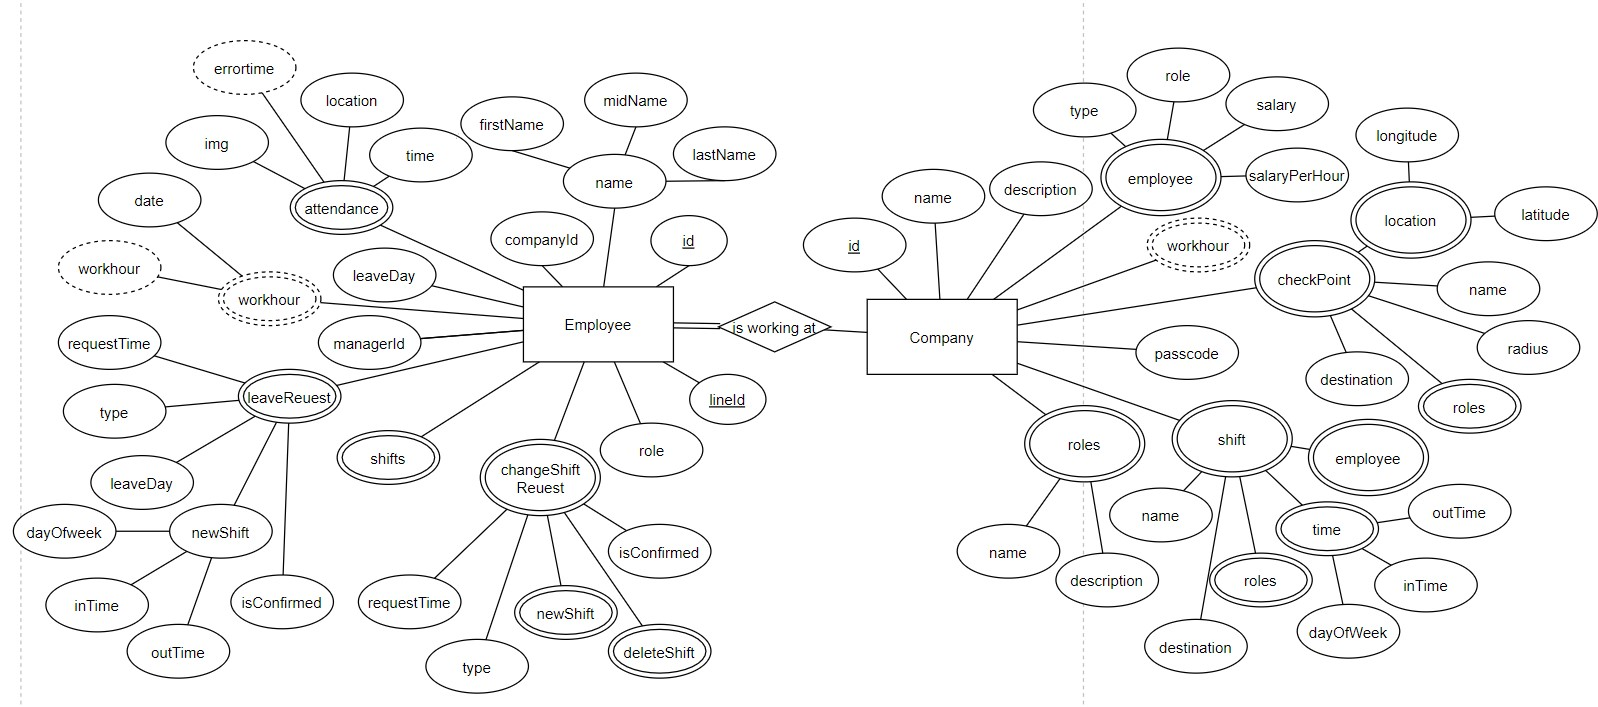
\includegraphics[width=14cm,keepaspectratio]{./images/ERdiagram.jpg}
\end{center}
\caption[Poem]{แสดง E-R Diagram(Entity-Relationship Diagram)ซึ่งแสดงรายละเอียดของข้อมูลของแต่ละ Entity ประกอบด้วย employee และ company}
\end{figure}

\begin{figure}
\begin{center}
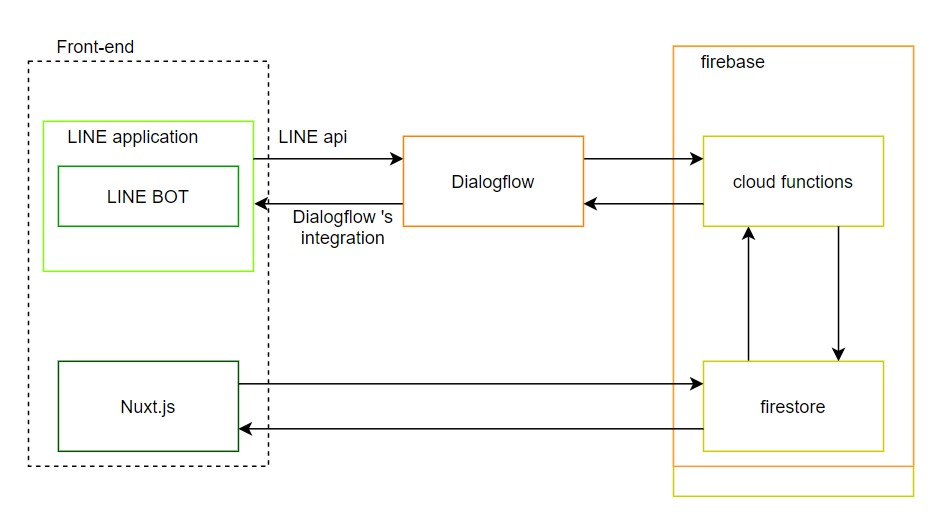
\includegraphics[width=14cm,keepaspectratio]{./images/structure.jpg}
\end{center}
\caption[Poem]{
  แสดงโครงสร้างของระบบ ซึ่งแบ่งเป็น 2 ส่วนใหญ่ ๆ คือ 
  Front-end ประกอบด้วย Line application(Line Bot) และ Nuxt.js 
  และ Back-end(firebase) ซึ่งประกอบด้วย firebase cloud functions และ firebase firestore 
  โดย มี dialogflow ขั้นกลางระหว่าง Line application และ firebase เพื่อทำหน้าที่แปลความหมายข้อความ
}
\end{figure}
\chapter{\ifproject%
\ifcpe การทดลองและผลลัพธ์\else Experimentation and Results\fi
\else%
\ifcpe การประเมินระบบ\else System Evaluation\fi
\fi}

ระบบที่ถูกพัฒนาขึ้นมาจะต้องสามารถทำได้ดังนี้ 

\section{การบันทึกเวลาเข้า-ออกของพนักงาน} 
ข้อมูลที่ถูกบันทึกต้องถูกต้องครบถ้วน เพื่อที่จะสามารถนำไปใช้ในการจัดการด้านต่าง ๆ และคำนวณเงินเดือนได้อย่างมีประสิทธิภาพ 

\section{การจัดการตารางเวลาทำงาน}
ข้อมูลที่ถูกบันทึกในตารางจะต้องถูกต้อง มีประสิทธิภาพ และเมื่อมีการเปลี่ยนแปลงตารางเวลาทำงานจะต้องมีการแจ้งเตือนไปยังเจ้าของตารางเพื่อให้รับรู้เข้าใจตรงกัน 

\section{ด้านความแม่นยำในการคำนวณเงินเดือน} 
ระบบต้องสามารถคำนวณได้ว่าเงินเดือนของพนักงานแต่ละคนเป็นเท่าใด โดยพิจารณาจากจำนวนชั่วโมงการทำงานของพนักงาน 

\ifproject
\chapter{\ifcpe บทสรุปและข้อเสนอแนะ\else Conclusions and Discussion\fi}

\section{\ifcpe สรุปผล\else Conclusions\fi}

นศ. ควรสรุปถึงข้อจำกัดของระบบในด้านต่างๆ ที่ระบบมีในเนื้อหาส่วนนี้ด้วย

\section{\ifcpe ปัญหาที่พบและแนวทางการแก้ไข\else Challenges\fi}

ในการทำโครงงานนี้ พบว่าเกิดปัญหาหลักๆ ดังนี้

\section{\ifcpe%
ข้อเสนอแนะและแนวทางการพัฒนาต่อ
\else%
Suggestions and further improvements
\fi
}

ข้อเสนอแนะเพื่อพัฒนาโครงงานนี้ต่อไป มีดังนี้

\fi

\bibliography{sampleReport}

\ifproject
\appendix
\chapter{The first appendix}

Text for the first appendix goes here.

\section{Appendix section}

Text for a section in the first appendix goes here.

\chapter{\ifcpe คู่มือการใช้งานระบบ\else Manual\fi}

Manual goes here.


%% Display glossary (optional) -- need glossary option.
\ifglossary\glossarypage\fi

%% Display index (optional) -- need idx option.
\ifindex\indexpage\fi

\begin{biosketch}
\begin{center}
  
\includegraphics[width=1.5in]{mugshot.jpg}
\end{center}
Your biosketch goes here. Make sure it sits inside
the \texttt{biosketch} environment.
\end{biosketch}
\fi % \ifproject
\end{document}
